\chapter{DHCP Configuration}

\section{Background}
\paragraph{}
Every machine, from computers to servers, requires an IP address
for it to be able to send and receive packets of data or information. (\cite{masterWS19})
These IP addresses act like home addresses on a street, and whilst DNS is 
responsible for resolving those IP addresses into names, there are two ways 
of assigning IP addresses to machines. These methods are static addressing
and DHCP (\cite{masterWS19}).

\paragraph{}
Static Addressing is the process of configuring IP addresses on a system
manually. It is a hands-on approach where IP addresses
are physically plugged into the NIC settings on a particular device (\cite{masterWS19}).
Despite its simplicity, this method is not scalable in environments that host
multiple devices like a small or large company, where there are laptops, desktops, 
printers, servers or other types of machines (\cite{masterWS19}). Each of these
devices needs an IP address, however manually assign them becomes tedious at a larger scale. The solution
to this problem lies in the Dynamic Host Configuration Protocol (DHCP) (\cite{masterWS19}).

\paragraph{}
DHCP is a protocol that solves the problem of providing IP addresses for many devices
on a wide scale. It allows for machines or devices that are plugged into the network and obtain 
IP address information (\cite{masterWS19}). This ability to assign IP address information to devices 
allows for DHCP to have multiple applications. When a laptop or phone is connected to a Wi-Fi router
to gain internet access, a DHCP server allows for that device to route traffic on the network by assigning
IP addressing information (\cite{masterWS19}). When a device connects to public Wi-Fi, its DHCP server runs on the router itself
and in businesses where Windows Server serves as a datacenter, DHCP services are most often hosted 
on one or more servers across the network (\cite{masterWS19}).

\section{Configuration Steps}
\subsection{The DHCP Scope}
\paragraph{}
For a DHCP server to hand out IP addresses, it needs to know IP addresses,
subnet mask, default gateway and DNS server addresses are within the network so that it can 
package and hand out the information to computers who request it. This package of information 
is called a DHCP scope (\cite{masterWS19}).

\paragraph{}
To begin defining the scope, we decided to launch a management tool using the Tools menu 
inside the Server Manager. This will open up a window for DHCP with the name of the device 
that the server is located on.
\begin{figure}[ht]
    \centering
    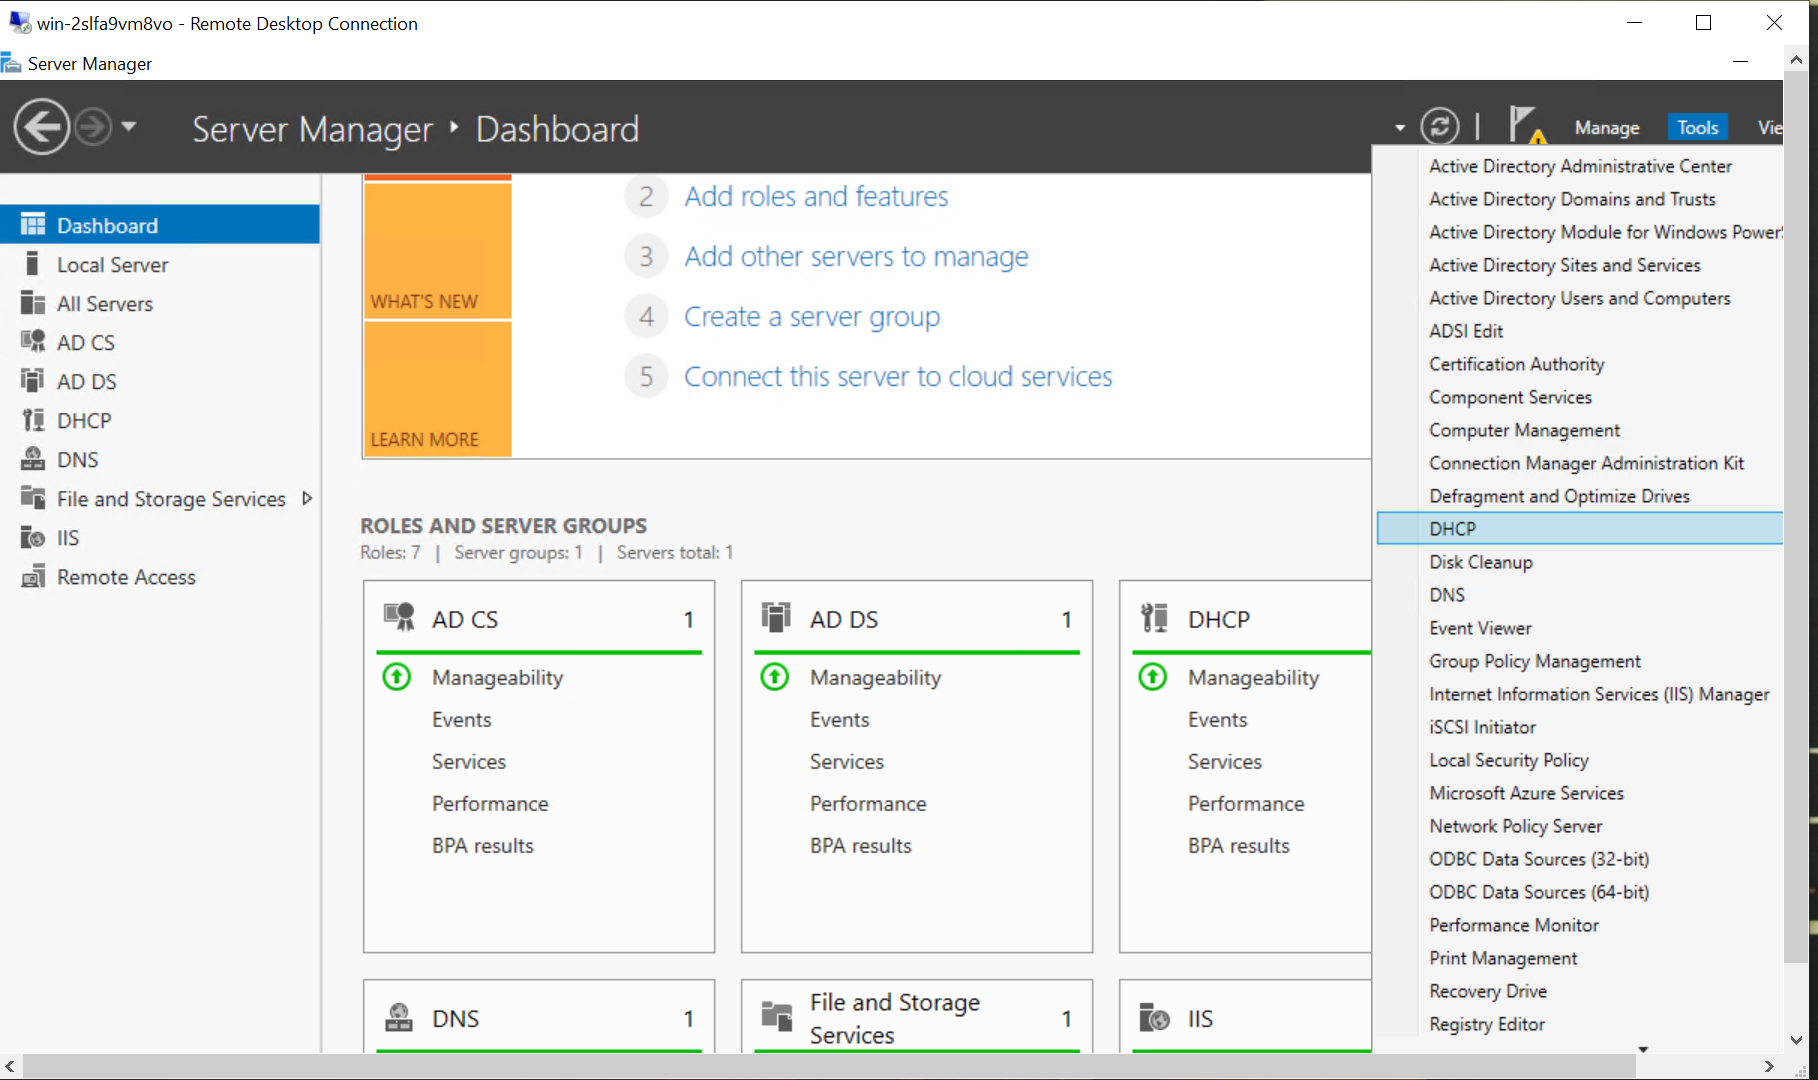
\includegraphics[width=0.7\linewidth]{Images/DHCP/Accessing DHCP through Tools Option.png}
    \caption{Accessing DHCP through Tools in Server Manager}
\end{figure}

\begin{figure}[ht]
    \centering
    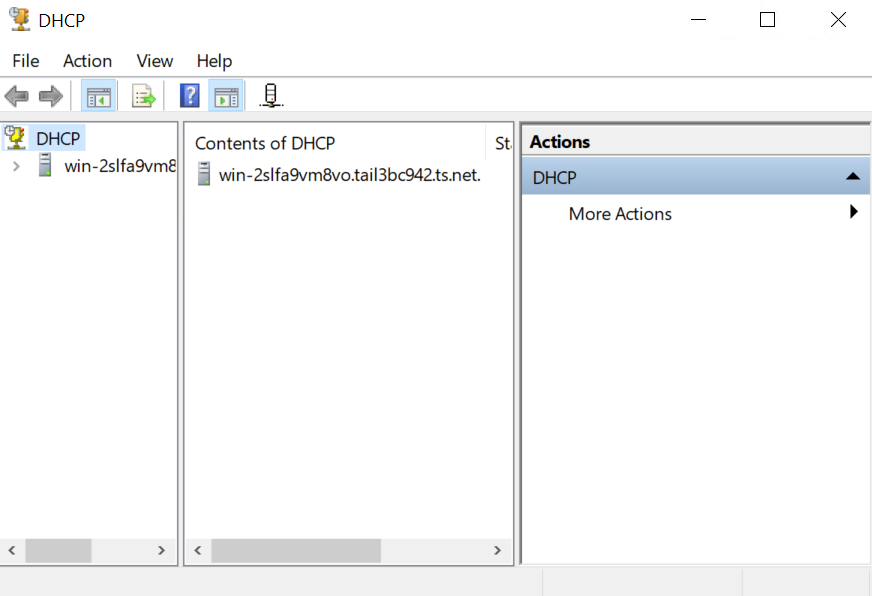
\includegraphics[width=0.7\linewidth]{Images/DHCP/DHCP window.png}
    \caption{DHCP window}
\end{figure}

\paragraph{}
After opening the DHCP window, the computer was selected and dropped down two protocols: IPv4 and IPv6.
The former was selected and first left-clicked on, where it gave information regarding the addition of a scope, along with the server 
options, policies and filters. This protocol did not have a scope as yet. 
To properly begin the process, IPv4 was right-clicked on, giving a drop-down menu when the option to add 
a new scope was present. Choosing this option opened the New Scope Wizard.

\begin{figure}[ht]
    \centering
    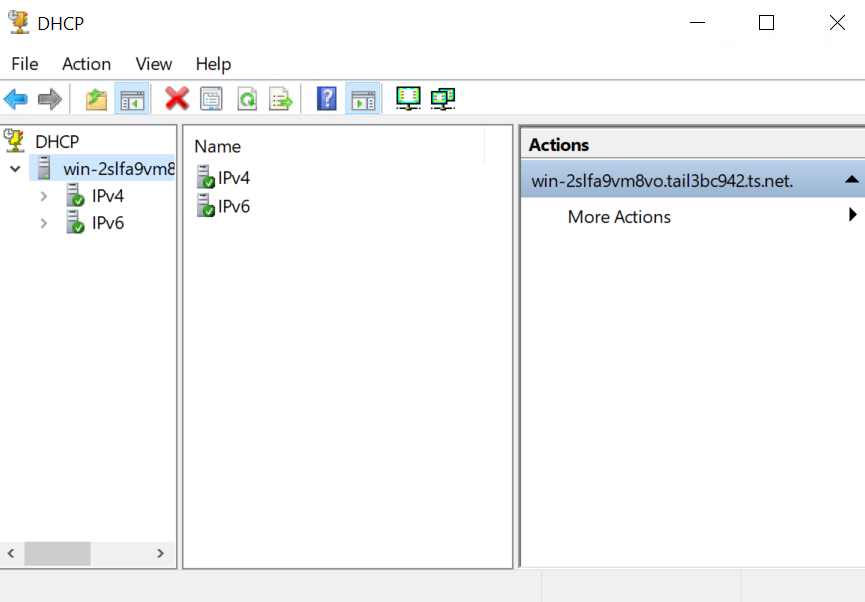
\includegraphics[width=0.7\linewidth]{Images/DHCP/Choosing an Internet Protocol.png}
    \caption{IPv4 and IPv6 available}
\end{figure}
\begin{figure}[ht]
    \centering
    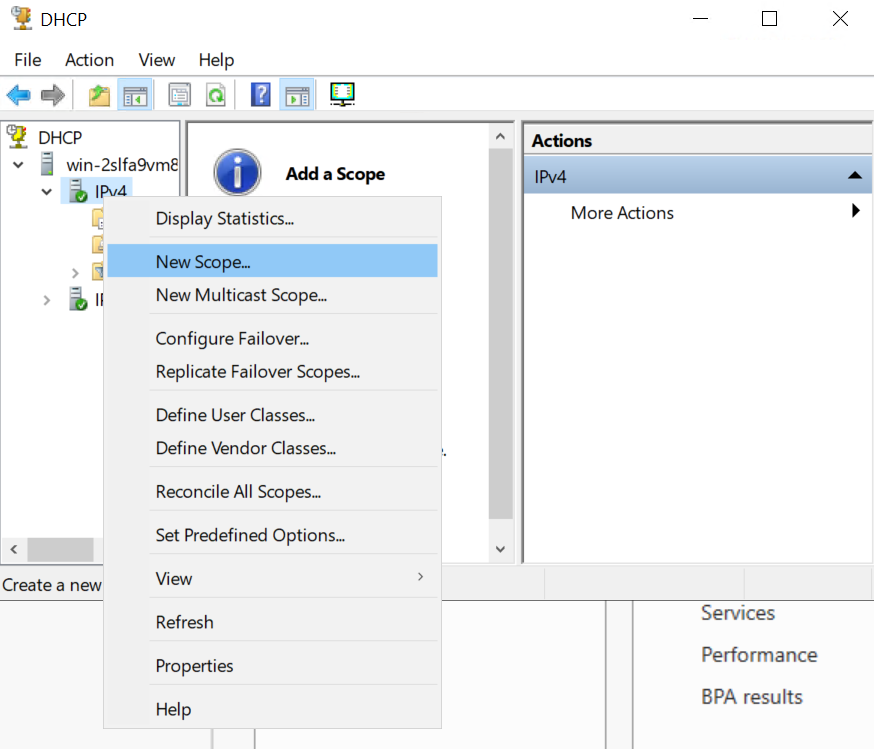
\includegraphics[width=0.7\linewidth]{Images/DHCP/Creating new Scope in IPv4.png}
    \caption{Creating new scope using IPv4}
\end{figure}
\begin{figure}[ht]
    \centering
    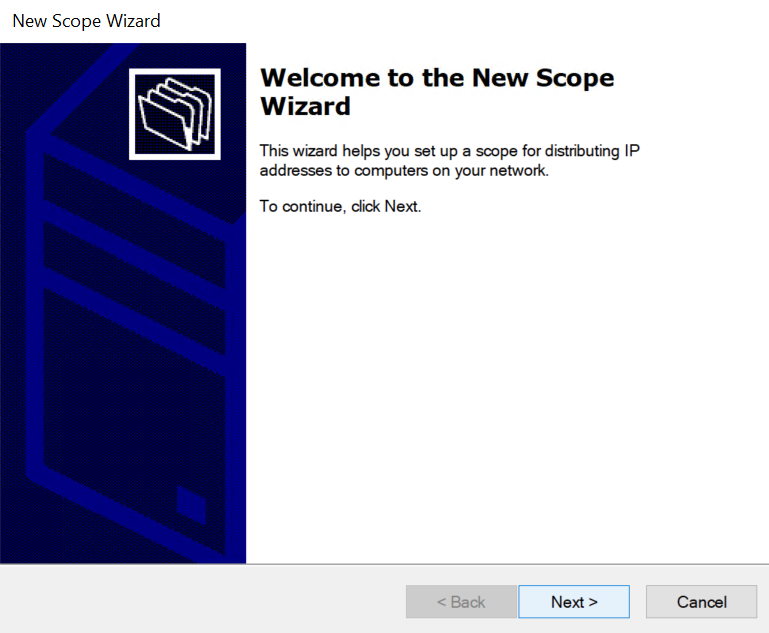
\includegraphics[width=0.7\linewidth]{Images/DHCP/New Scope Wizard.png}
    \caption{New Scope Wizard}
\end{figure}